%======================================================================
\chapter{Mechanism of \texorpdfstring{\ce{CO2}}{CO2} Reduction}\label{chap.mech}
\markright{Computational Study of the Mechanism of \texorpdfstring{\ce{CO2}}{CO2} Reduction}
%======================================================================

%======================================================================
\section{Introduction}
%======================================================================

Within three years of the originally reported bipyridine rhenium I catalyst, experimental studies on the mechanism of the photocatalytic reduction of \ce{CO2} were available in the literature\autocite{hawecker1986}. Studies continue on the mechanism up to the present day\autocite{koike2002, machan2014}\todo{more}, utilizing new investigative techniques as they become available. Investigation includes the use of \gls{ac.dft} methods to elucidate geometries of intermediates and transition states for of the multi-step cycle. Transition metal catalysis is a non-trivial problem computationally, especially when considering a metal from the lower period. These elements contain a large amount of electrons, many of which can be involved in non-covalent interactions with the ligands and catalyzed products. Solving for this complex system becomes non-trivial and computationally expensive. For this reason, no overview of the mechanism as investigated by \gls{ac.dft} methods has ever been made available in the literature. 

%======================================================================
\section{Literature Mechanism Pathways}
%======================================================================

Prior work in the literature has proposed three general mechanistic pathways for the photoreduction of \ce{CO2}. In general, as seen in \autoref{fig.threepath}, these pathways result in the formation of \ce{CO} and \ce{H2O}, formate (\ce{HCO2-}), or carbonate (\ce{CO3H-}) anions. The formation of carbonate proceeds via the formation of a catalyst dimer over a molecule of \ce{CO2}, with the insertion of a second molecule of \ce{CO2} to produce the carbonate and a molecule of \ce{CO}. Formation of formate occurs via insertion of \ce{CO2} to a rhenium hydride bond. The formation of \ce{CO} without carbonate or formate by-products occurs via the coordination of \ce{CO2} to an open site on the metal, followed by a double proton addition and the release of a molecule of \ce{H2O} prior to the loss of one of the four carbonyl groups to open up the axial site for halide re-coordination. This is essentially the \gls{ac.rwgsr}, wherein protons are made available from decomposition of the sacrificial amine instead of from \ce{H2} gas\autocite{kalyanasundaram1978}. The activation of the catalyst with respect to radicalization, electron abstraction from the sacrificial reductant, and anion disassociation is well studied, the character of the \ce{CO2} adduct is less well known. These three mechanistic pathways will be referred to as the `carbonate' mechanism, the `formate' mechanism, and the `water-gas shift' mechanism, respectively.

\begin{figure}[!htb]
 \begin{center}
  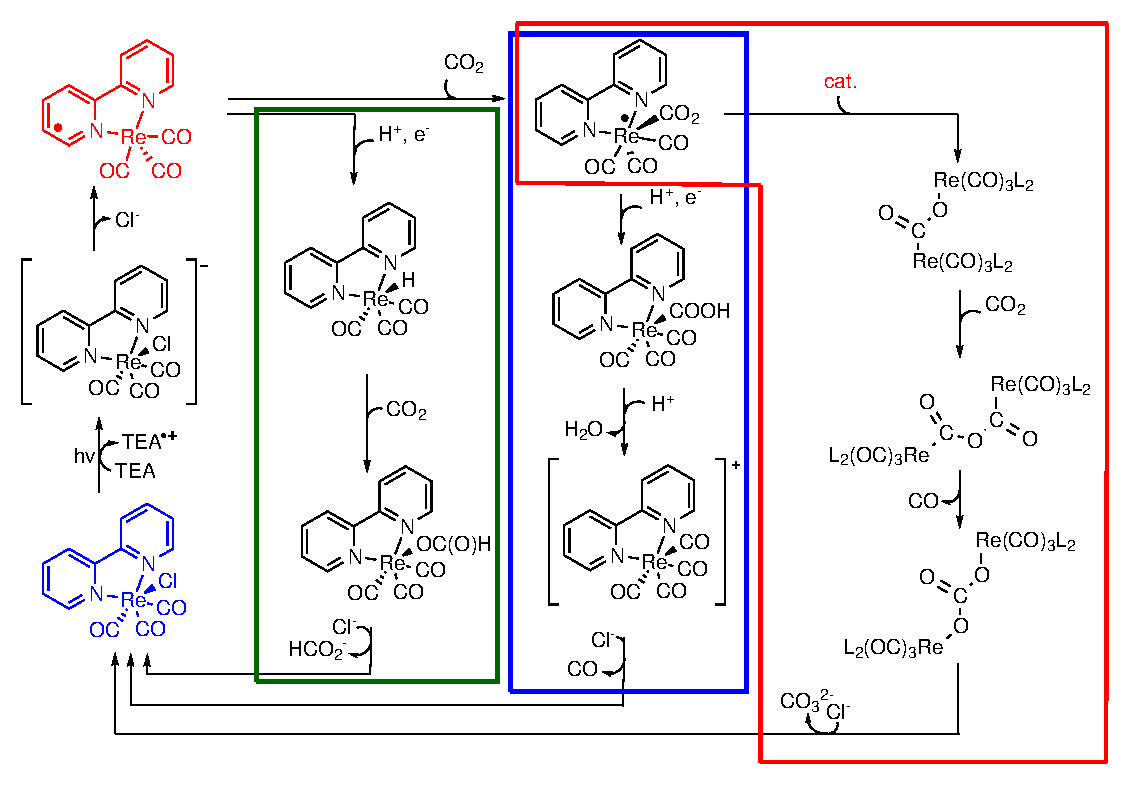
\includegraphics[clip=true, width=\textwidth, keepaspectratio]{images/threepaths.eps}
 \end{center}
\caption[Overview of mechanistic pathways]{An overview of the mechanistic pathways of photochemical \ce{CO2} reduction. Catalyst is shown in blue, and the excimer species in red}
\label{fig.threepath}
\end{figure} 

All of the pathways require the formation of a common eximer species, namely, the radical 17\textit{e}\textsuperscript{-} species (\autoref{fig.eximer}). This occurs through the absorption of an incident photon with enough energy to promote an electron from the metal d-orbital to the ligand $\pi^\ast$ orbitals in the ground state catalyst, \textbf{4.01}. The pseudo-oxidized, electron-deficient metal atom extracts an electron from the sacrificial amine (\textbf{4.05}) to return to the \ce{Re^{I}} state (\textbf{4.02}). However, this complex is formally a radical anion, the halide (\textbf{4.04}) is lost to return to the neutral eximer species in solution, \textbf{4.03}. 

\begin{figure}[!htb]
 \begin{center}
  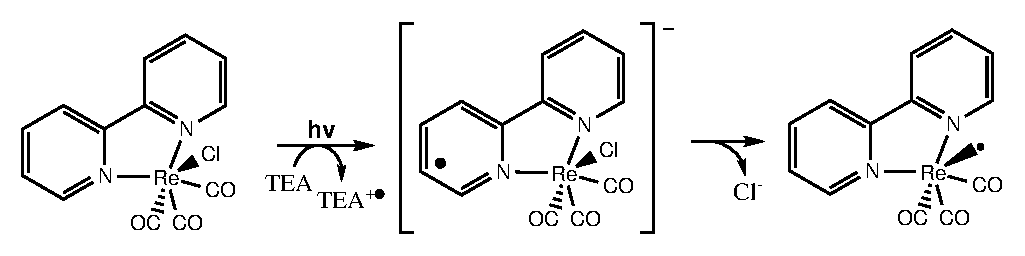
\includegraphics[clip=true, width=120mm, keepaspectratio]{images/eximer.eps}
 \end{center}
\caption{Formation of the eximer species via absorption of a photon and oxidation of the sacrificial amine.}
\label{fig.eximer}
\end{figure} 

The decomposition of the sacrificial amine was first identified by \todo{ref}, and is summarized in \autoref{fig.decomp}. This decomposition is important because of the protons it provides to the reaction mixture, and the ease of second electron abstraction from a decomposition product. The radical cationic species (\ce{Et3N^{+.}}, \textbf{4.06}) undergoes a proton transfer to a second molecule of the sacrificial reductant. The transfer removes a proton from the $\alpha$ carbon, leaving it a radical species but removing the charge (\textbf{4.07}). This species is able to react in the catalytic cycle to provide a second electron and form the ethene-diethylamino compound. Triethylammonia is produced as well (\textbf{4.08}), this is a proton source for other mechanistic steps.

\begin{figure}[!htb]
 \begin{center}
  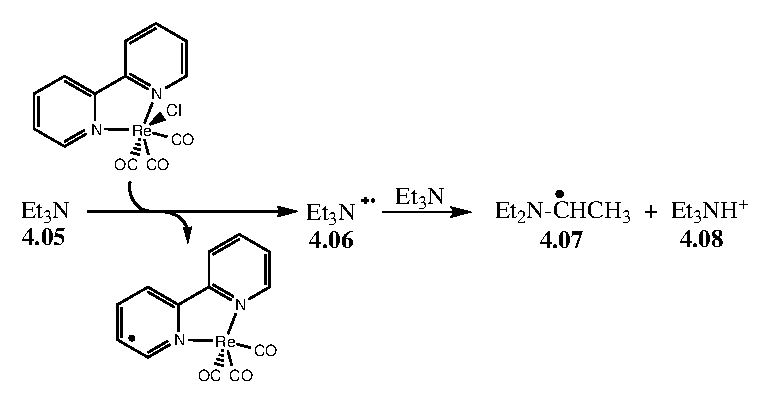
\includegraphics[clip=true, width=100mm, keepaspectratio]{images/reddecomp.eps}
 \end{center}
\caption{Decomposition pathway for the sacrificial amine.}
\label{fig.decomp}
\end{figure} 

Each of the mechanistic pathways identified above in \autoref{fig.threepath} was studied, using \gls{ac.dft} methods. Structures (using 2,2'-bipyridine as the bidentate ligand, and triethylamine as the sacrificial reductant) were optimized to ground or transition states using TurboMole 6.5\autocite{turbomole, ahlrichs1989}, with the TPSS meta-GGA XC functional\autocite{tao2003}. The def2-TZVP basis set was used for all atoms\autocite{schafer1994, weigend2005}. The TurboMole program contains a number of optimizations to the original \gls{ac.dft} algorithms\autocite{haase1993, treutler1995, eichkorn1997, eichkorn1995, sierka2003, deglmann2004, weigend2002, vonarnim1998, ahlrichs2004}, decreasing the calculation time without compromising accuracy. Grimme's dispersion correction (version 3) was included in the calculations\autocite{grimme2010}. Intermediates and transition states were verified by frequency analysis\autocite{deglmann2004, deglmann2002, grimme2002}, with further verification of transition states by performing dynamic reaction coordinate calculations to determine the \glspl{ac.irc}. The effects of solvation was calculated using the Conductor-like Screening Model (COSMO) implemented in TurboMole\autocite{klamt1993}, which is a continuum solvation model implicitly surrounding the solute molecule. Code was developed to assist with managing the computational jobs (see \autoref{chap.turbocontrol}).

Many of the intermediates have been synthesized in various studies \todo{Refs. Sullivan and Gilbert}, indicating their reasonable stability. While individual portions of the mechanism have been studied computationally in the past\todo{refs}, no over-arching study has compared methods relative to each other. Furthermore, while the formation of \ce{CO} with \ce{H2O} is the most anticipated pathway (due to the lack of formation of carbonate or formate in most studies), no literature pathway exists to explain the addition of \ce{CO2} to the open site of the radical catalytic species without a three body reaction step (catalyst, \ce{CO2} and \ce{H+} together) or without formate reorganization. Furthermore, no mechanism proposed thus far explains the \ce{^{12}CO} to \ce{^{13}CO} isotopic exchange demonstrated by Lehn's group in 1986\autocite{hawecker1986}. 

%---------------------------------------------------------------------
\subsection{Eximer Formation and Decomposition of the Sacrificial Amine}\label{ss.initiation}
%---------------------------------------------------------------------

Each of the mechanisms described require the activation of the catalyst prior to \ce{CO2} reduction (see \autoref{fig.decomp} and \autoref{fig.eximer}). Catalyst is solvated with large excess of \gls{ac.tea} or \gls{ac.teoa} available. Incoming photons promote an electron from the metal \textit{d}-orbital centred \gls{ac.homo} to the ligand $\pi^\ast$-style \gls{ac.lumo}. This promotion forms an electron-poor metal centre of the complex, which is able to extract a proton from the amine. This extraction to form the radical anion catalyst and the radical cation is surprisingly favoured by a significant amount both in the gas phase (-39.27 kcal/mol) and in simulated DMF (-67.83 kcal/mol), when using bipyridine catalysts and a triethylamine sacrificial agent.

Energies of \textbf{4.01} - \textbf{4.10}, and \textbf{4.26} in gas and solution phases (in \gls{ac.dmf}) is shown in \autoref{tab.supenergy}, along with the energy of solvation. %Reaction energies are listed in \autoref{tab.suprxn}.

% Table generated by Excel2LaTeX
\begin{table}[!htb]
\centering
 \begin{threeparttable}
  \caption[Gas phase and solvated energies for mechanism reactants and products]{Gas phase and solvated energies of mechanism reactants and products.}
    \begin{tabular}{llrrr}
    \toprule
    Molecule & Label & E (gas)\tnote{a} & E (solution)\tnote{b} & E (solvation)\tnote{c} \\
    \midrule
    Ground State & \textbf{4.01} & -1374.621419 & -1374.651099 & 18.62 \\
    3MLCT Complex & textbf{\textsuperscript{3}4.01\textsuperscript{MLCT}} & -1374.553193 & -1374.565998 & 8.04 \\
    Radical Anion & \textbf{4.02} & -1374.684002 & -1374.759190 & 47.18 \\
    Open Site Excimer & \textbf{4.03} & -914.3139376 & -914.3287245 & 9.28 \\
    Chlorine Anion & \textbf{4.04} & -460.2890817 & -460.4058583 & 73.28 \\
    Triethylamine (TEA) & \textbf{4.05} & -292.3051496 & -292.3854033 & 50.36 \\
    Radical Cation TEA & \textbf{4.06} & -292.3051496 & -292.3854033 & 50.36 \\
    Deprotonated TEA Radical & \textbf{4.07} & -291.9173706 & -291.9211226 & 2.35 \\
    Triethylammonia & \textbf{4.08} & -292.9552538 & -293.0382729 & 52.09 \\
    Carbon Dioxide & \textbf{4.09} & -188.6945676 & -188.6974631 & 1.82 \\
    Carbon Monoxide & \textbf{4.10} & -113.3744946 & -113.3754466 & 0.60 \\
    Diethylaminoethene & \textbf{4.26} & -291.3467768 & -291.3525868 & 3.64 \\
    \bottomrule
    \end{tabular}%
    \begin{tablenotes}
    \item [a] TPSS energy in hartrees.
    \item [b] TPSS energy in hartrees with COSMO solvation in DMF.
    \item [c] TPSS solvation energy in kcal/mol (E(gas) - E(solution)).
    \end{tablenotes}
  \label{tab.supenergy}%
 \end{threeparttable}
\end{table}%



%% Table generated by Excel2LaTeX
\begin{table}[!htb]
\centering
 \begin{threeparttable}
  \caption{Energies for the reaction steps in the photoinduced excimer formation pathway}
    \begin{tabular}{r@{ $\rightarrow$ }lrr}
    \toprule
    \multicolumn{2}{c}{Steps} & Energy(gas)\tnote{a} & Energy(dmf)\tnote{b} \\
    \midrule
    \textbf{4.01} & \textbf{\textsuperscript{3}4.01\textsuperscript{MLCT}} & 42.81 & 53.40 \\
    \textbf{4.01\textsuperscript{3MLCT}} + \textbf{4.05} & \textbf{4.02} + \textbf{4.06} & 81.45 & -5.80 \\
    \textbf{4.02} & \textbf{4.03} + \textbf{4.04} & 50.82 & 15.44 \\
    \textbf{4.06} + \textbf{4.05} & \textbf{4.07} + \textbf{4.08} & -1.08 & -2.92 \\
    \bottomrule
    \end{tabular}%
    \begin{tablenotes}
    \item [a] TPSS energy in kcal/mol.
    \item [b] TPSS energy in kcal/mol with COSMO solvation in DMF.
    \end{tablenotes}
  \label{tab.suprxn}%
 \end{threeparttable}
\end{table}%




The further decomposition of the amine via proton extraction to a second molecule to form the neutral radical and the tetra-coordinate amine is significantly favoured (> than 100 kcal/mol in both gas and solvated situations). A slight uphill to dissociation of the chloride (15.44 kcal/mol in DMF) allows for the formation of the triplet 17 \textit{e}$^-$ excimer species, from which the following mechanisms may progress.

%---------------------------------------------------------------------
\subsection{The `Carbonate' Pathway}\label{ss.carbonate}
%---------------------------------------------------------------------

The carbonate pathway is shown in \autoref{fig.carbonate}, starting from the excimer species. In this reaction, two molecules of the excimer species (\textbf{4.03}) combine over a molecule of \ce{CO2} (\textbf{4.09}), forming a stable intermediate where one catalyst molecule is bound to the central carbon atom of the gas, while the other is bound to one of the pendant oxygen atoms (\textbf{4.11}). A second molecule of \ce{CO2} is inserted into the oxygen-rhenium bond, forming \textbf{4.12}. The transition state is a loose four membered ring with the rhenium atom, the oxygen from the first \ce{CO2} molecule, and the carbon and one oxygen atom from the new incoming molecule. This four-membered ring breaks apart to relax to a \ce{\bond{-}OC(O)OC(O)\bond{-}} linked catalyst dimer (\textbf{4.13}). The \ce{CO2} reduction continues via another rearrangement to form a five-membered ring transition state \textbf{4.14}, resulting in the release of a \ce{CO} molecule (\textbf{4.10}) and the formation of a carbonate (\ce{\bond{-}OC(O)O\bond{-}}) linker (\textbf{4.15}). Dissociation of this yielding the carbonate catalyst \textbf{4.16}, and the re-addition of halide to the molecule results in the formation of the catalyst ground states \textbf{4.01} and the bicarbonate anion \textbf{4.17}.

\begin{figure}[!ht]
 \begin{center}
  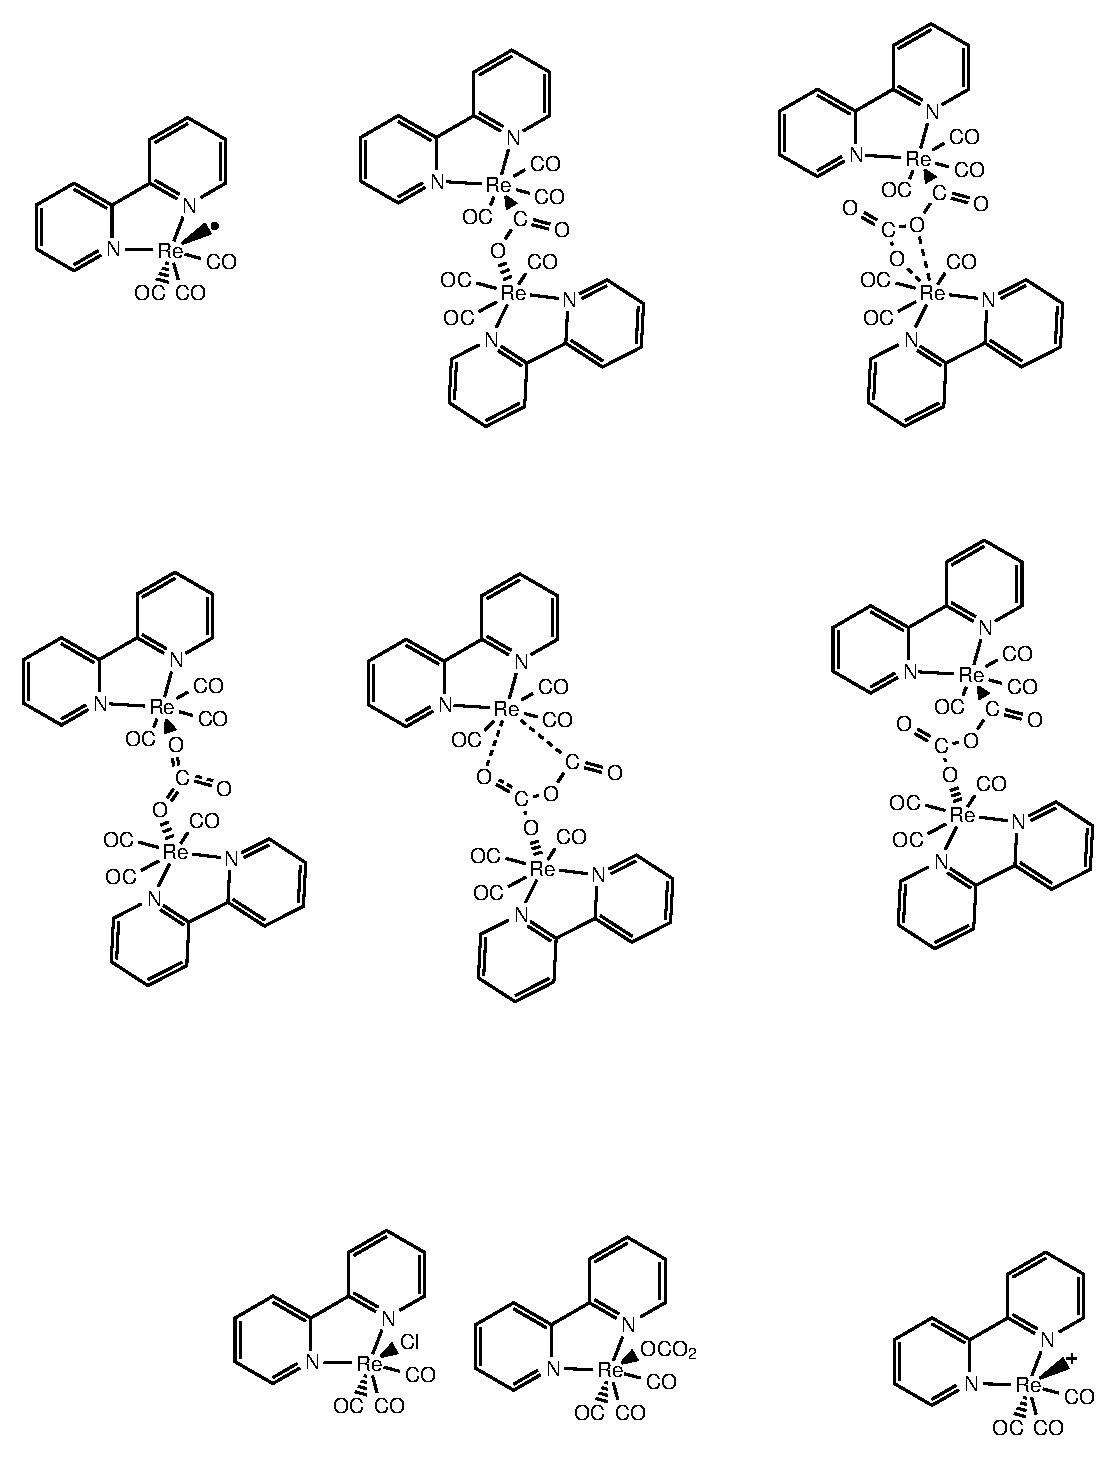
\includegraphics[clip=true, width=140mm, keepaspectratio]{images/carbonate.eps}
 \end{center}
\caption{The `carbonate' mechanistic pathway}
\label{fig.carbonate}
\end{figure} 

Energies of each of the compounds involved in this mechanism pathway are shown in \autoref{tab.carbenergy}, along with the energy of solvation. The full list of reaction energies are listed in \autoref{tab.carbrxn}.

% Table generated by Excel2LaTeX
\begin{table}[!htb]
\centering
 \begin{threeparttable}
  \caption[Gas phase and solvated energies for the `carbonate' mechanism]{Gas phase and solvated energies of compounds, transition states and intermediates in the `carbonate' mechanism}
    \begin{tabular}{llrrr}
    \toprule
    Molecule & Label & E (gas)\tnote{a} & E (solution)\tnote{b} & E (solvation)\tnote{c} \\
    \midrule
    \ce{CO2} Linked Dimer & 4.11 & -2017.373132 & -2017.412314 & 24.59 \\
    \ce{CO2} Addition TS & 4.12 & -2206.120721 & -2206.165017 & 27.80 \\
    \ce{C2O4} Linked Dimer & 4.13 & -2206.047558 & -2206.097328 & 31.23 \\
    5 Member Ringed Dimer TS & 4.14 & -2206.013925 & -2206.061531 & 29.87 \\
    \ce{CO3} Linked Dimer & 4.15 & -2092.678255 & -2092.725669 & 29.75 \\
    Bicarbonate Catalyst Cation & 4.16 & -1178.065153 & -1178.119717 & 34.24 \\
    Bicarbonate Anion & 4.17 & -264.4852375 & -264.4967144 & 7.20 \\
    Dimer Formation TS & 4.18 & -2017.434125 & -2017.47423151664 & 25.17 \\
    Bicarbonate Dianion & 4.19 & -263.7946209 & -264.1983931 & 253.37 \\
    Open Site Cation & 4.27 & -914.1064097 & -914.1872844 & 50.75 \\
    \bottomrule
    \end{tabular}%
    \begin{tablenotes}
    \item [a] TPSS SCF energy in hartrees.
    \item [b] TPSS SCF energy in hartrees with COSMO solvation in DMF.
    \item [c] TPSS solvation energy in kcal/mol (E(gas) - E(solution)).
    \end{tablenotes}
  \label{tab.carbenergy}%
 \end{threeparttable}
\end{table}%



% Table generated by Excel2LaTeX
\begin{table}[!htb]
\centering
 \begin{threeparttable}
  \caption{Energies for the reaction steps in the `formate' pathway}
    % Table generated by Excel2LaTeX from sheet 'Tex Charts
    \begin{tabular}{rrrr}
    \toprule
    Description & Steps & Energy(gas)\tnote{a} & Energy(dmf)\tnote{b} \\
    \midrule
    Formation of Radical Anion & 4.01, 4.05 \ce{->} 4.02, 4.06   & 124.261582 & 47.596907 \\
    Open site catalyst plus cl- & 4.02 \ce{->} 4.03, 4.04 & 50.816912 & 15.440887 \\
    Reconfiguration of TEA & 4.06, 4.05 \ce{->} 4.07, 4.08 & -1.077024 & -2.915901 \\
    \midrule
    Addition of CO2 to open site & 4.4   & -0.2501423 & 6.37310903 \\
    addition of second cat to CO2 & 4.5   & 118379.026 & 118375.044 \\
    Insertion of CO2 & 4.6   & \#VALUE! & -8.5491267 \\
    relaxation of co2 insertion & 4.7   & \#VALUE! & -0.6637971 \\
    rearrange to 4ring dimer & 4.8   & \#VALUE! & \#VALUE! \\
    relax to long & 4.9   & \#VALUE! & \#VALUE! \\
    rearrangement to 5ring dimer & 4.1   & \#VALUE! & 22.4628711 \\
    relax to final & 4.11  & \#VALUE! & -24.839557 \\
    break apart & 4.12  & 317.951051 & 262.714812 \\
    return to ground states & 4.13  & -613.91666 & -426.82371 \\
    \bottomrule
    \end{tabular}%
    \begin{tablenotes}
    \item [a] TPSS SCF energy in kcal/mol.
    \item [b] TPSS SCF energy in kcal/mol with COSMO solvation in DMF.
    \end{tablenotes}
  \label{tab.carbrxn}%
 \end{threeparttable}
\end{table}%


The entirety of this pathway has not been studied in the literature previously. Analysis of the central portion of the pathway, from the formed \ce{CO2} linked dimer, through the release of \ce{CO}, terminating at the bicarbonate linked dimer. The study built the dimer as a three-body reaction, with a \ce{Re\bond{-}Re} bound catalyst dimer, and did not discuss the decomposition to the catalyst ground states. 

The mechanism starts with the addition of a \ce{CO2} molecule to the excimer. This is a very weakly bound species when solved in a simulated \gls{ac.dmf} environment; in the gas phase this transition complex will not solve. The \gls{ac.dmf} solved structure has a Re-C bond length of 2.50654 \r{A}, and O-C-O bonding angle of 142$^\circ$. Compared to the \ce{Re\bond{-}C} distances of \textit{ca}. 1.9 \r{A}; this is a very weakly coordinated bond. The formation of this `bond' requires only 6.37 kcal/mol, the radical species is not satisfied with the addition of \ce{CO2} and  This unstable complex is able to extract a proton to continue with the formate pathway (see below \autoref{ss.formate}), or combine with a second molecule of the excimer to form a dimer. This dimer formation is explicitly not favoured; although resolution of radical species is provided, the transformation is still \todo{numb} uphill. Explanation of this untenably large value may be the root of the choice in literature to utilize the Re-Re bound dimer species as the catalyst starting point, instead of the ground state. From this point onwards the reaction proceeds in achievable downhill steps, the formation of the dimer is the rate limiting step for the entire reaction pathway. 

Following the insertion of a second molecule of \ce{CO2}, a number of internal rearrangements are required. These steps are outlined in \todo{numbers}. This rearrangement moves from a linear chain of oxygen and carbon atoms to a bicarbonate, with the release of \ce{CO} observed. The resulting dimer species is left to decompose to a catalyst cation with an open site, and the bicarbonate adduct. This carbonate dianion may pick up a proton before or after the disassociation to the catalyst cationic species, resulting in the released of the bicarbonate species to solution. 

Some work done by Agarwal \textit{et. al.} provides an opportunity for a catalytic pathway with similar results requiring only one molecule of catalyst. Instead of capping the loosely coordinated \ce{CO2} with the eximer, the radical is quenched with a hydride extraction from the sacrificial amine, much as in the pathway described in \autoref{ss.formate}. A second molecule of \ce{CO2} reacts with the acid, undergoing a series of steps to produce the carbonate. The experimental data supporting this variation of the mechanism is not strong, further validation should be required for this variation to gain traction in the literature. 

\FloatBarrier

%---------------------------------------------------------------------
\subsection{The `Formate' Pathway}\label{ss.formate}
%---------------------------------------------------------------------
In comparison to the catalytic dimer formed in the carbonate pathway above, the formate formation occurs via a much simpler mechanism. The addition of a proton to the open site axial to the ligand occurs via the simultaneous electron and proton transfer from a by-product of the reduction of the amine. \ce{CO2} inserts into this metal hydride bond, resulting in a metal-oxide bond, with the formate anion. Separation of the weak metal-oxygen bond allows for the reinsertion of the halide to the cationic metal centre. 

\begin{figure}[!htb]
 \begin{center}
  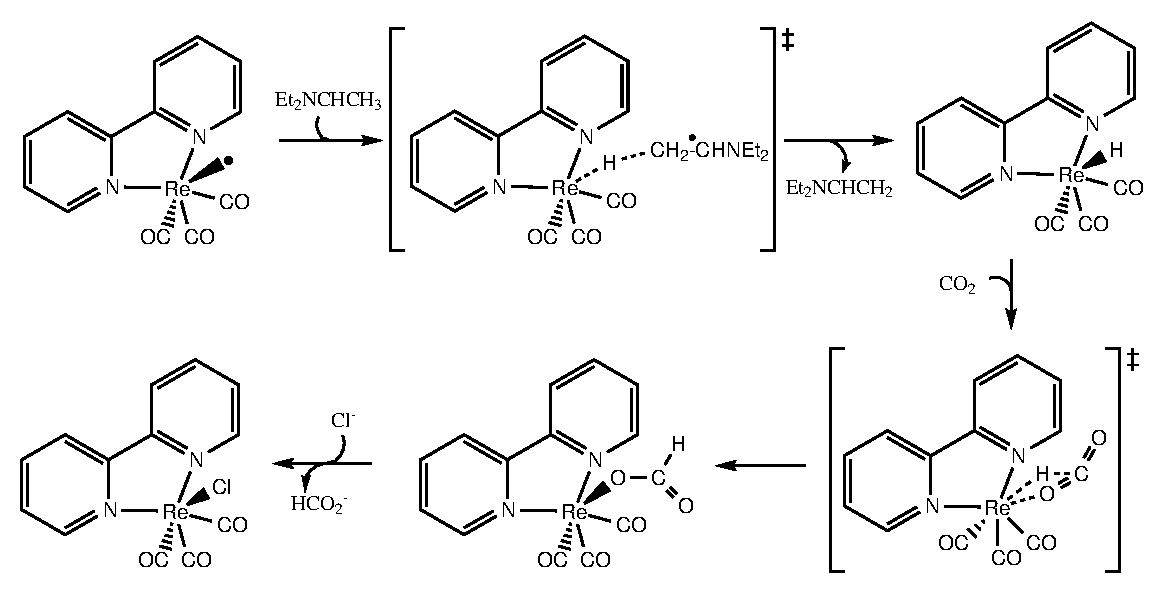
\includegraphics[clip=true, width=\textwidth, keepaspectratio]{images/formate.eps}
 \end{center}
\caption{The `formate' mechanistic pathway}
\label{fig.formate}
\end{figure} 

Energies of each of the compounds involved in this mechanism pathway are shown in \autoref{tab.formenergy}, along with the energy of solvation.

% Table generated by Excel2LaTeX
\begin{table}[!htb]
\centering
 \begin{threeparttable}
  \caption[Gas phase and solvated energies for the `formate' mechanism]{Gas phase and solvated energies of compounds, transition states and intermediates in the `formate' mechanism}
    \begin{tabular}{llrrr}
    \toprule
    Molecule & Label & E (gas)\tnote{a} & E (solution)\tnote{b} & E (solvation)\tnote{c} \\
    \midrule
    Proton Transfer TS & 4.21  & -1206.302997 & -1206.32707 & 15.10 \\
    Catalyst Hydride & 4.22  & -914.9204746 & -914.9448354 & 15.29 \\
    \ce{CO2} Insertion TS & 4.23  & -1103.581201 & -1103.619960 & 24.32 \\
    Catalyst Formate & 4.24  & -1103.635283 & -1103.665628 & 19.04 \\
    Formate Anion & 4.25 & -189.3051464 & -189.4151284 & 69.01 \\
    Open Site Cation & 4.27  & -914.1064097 & -914.1872844 & 50.75 \\
    \bottomrule
    \end{tabular}%
    \begin{tablenotes}
    \item [a] TPSS SCF energy in hartrees.
    \item [b] TPSS SCF energy in hartrees with COSMO solvation in DMF.
    \item [c] TPSS solvation energy in kcal/mol (E(gas) - E(solution)).
    \end{tablenotes}
  \label{tab.formenergy}%
 \end{threeparttable}
\end{table}%



% Table generated by Excel2LaTeX
\begin{table}[!htb]
\centering
 \begin{threeparttable}
  \caption{Energies for the reaction steps in the `formate' pathway}
    % Table generated by Excel2LaTeX from sheet 'Tex Charts
    \begin{tabular}{rrrr}
    \toprule
    Description & Steps & Energy(gas)\tnote{a} & Energy(dmf)\tnote{b} \\
    \midrule
    Formation of Radical Anion & 1.1   & -39.271301 & -67.827267 \\
    Open site catalyst plus cl- & 1.2   & 50.8169125 & 15.4408871 \\
    Reconfiguration of TEA & 1.3   & -164.60991 & -118.34007 \\
    \midrule
    Hydride Extraction & 1.4   & 4.09794743 & -9.8319638 \\
    Removal of TEA & 1.5   & -26.652434 & -20.021496 \\
    Insertion of CO2 & 1.6   & 21.2356096 & 14.0177223 \\
    recoordination & 1.7   & -33.936535 & -28.657394 \\
    dissasotiation of HCO2- & 1.8   & 140.389052 & 39.6680755 \\
    Reformation of Catalyst & 1.9   & -141.76995 & -36.367745 \\
    \bottomrule
    \end{tabular}%
    \begin{tablenotes}
    \item [a] TPSS SCF energy in kcal/mol.
    \item [b] TPSS SCF energy in kcal/mol with COSMO solvation in DMF.
    \end{tablenotes}
  \label{tab.formrxn}%
 \end{threeparttable}
\end{table}%



After formation of the excimer \textbf{4.03}, the radical species extracts a hydrogen atom from the oxidized chain of the sacrificial amine \textbf{4.07}, a step with a barrier of -9.83\todo{update with new value} kcal/mol in DMF. The sacrificial amine involved in this step had previously had one proton extracted by another molecule of the amine in a proton exchange step (see \autoref{ss.initiation}), resulting in a neutral radical. Extraction of the proton and electron pair allows for the formation of an ethene arm, completing the decomposition of the amine to the final neutral, singlet molecule \textbf{4.26}. Relaxation of this transition state results in the hydrogen extraction from the radical species, yielding the formation of the hydride complex \textbf{4.22}. 

This hydride complex is able to insert a molecule of \ce{CO2} into the metal-hydrogen bond, in transition step \textbf{4.23}. While typically seen in other organo-metal chemistries, rhenium(I) hydrides are very rare, only appearing as intermediates in these mechanisms. The Re-H bond length is \todo{length} \r{A}, compared to the length of the Re-Cl bond from the ground state \textbf{4.01} species. When a molecule of \ce{CO2} approaches, the transition state of a pseudo-septa-coordinate species forms. The formation is expensive, at just over 14 kcal/mol. The Re-H bond increases in length to \r{A}, the Re-O bond is \r{A}, and the O-Re-H angle remains tight at $^\circ$. This step completes with 28.66 kcal/mol energy release to form the formato anion complex \textbf{4.24}. 

The formato anion \textbf{4.25} dissociates with a chloride re-entry requiring less than 3 kcal/mol for the dissociation. This counterion exchange is likely more favoured in the real solution, not all contributions from products and the electrolyte are included in the calculation. Further reactions of the formato anion in solution are not investigated, but the anion likely remains deprotonated in the slightly basic environment. 

\FloatBarrier

%---------------------------------------------------------------------
\subsection{The `Water-Gas Shift' Pathway}\label{ss.watergas}
%---------------------------------------------------------------------
The water-gas shift mechanism involves the addition of two protons from the reductant to a \ce{CO2} molecule bound to the metal centre. The first proton addition yields an acid species, this is dehydrated via the second addition of a proton and the release of one molecule of \ce{H2O}. The resulting tetracarbonyl cationic species is able then to release an axial carbonyl to return to the ground state. While any of the carbonyl groups could be labile, the carbonyl at the axial position is the one actively replaced by the halide to return to the starting catalyst\autocite{shaver1992}. 

\begin{figure}[!htb]
 \begin{center}
  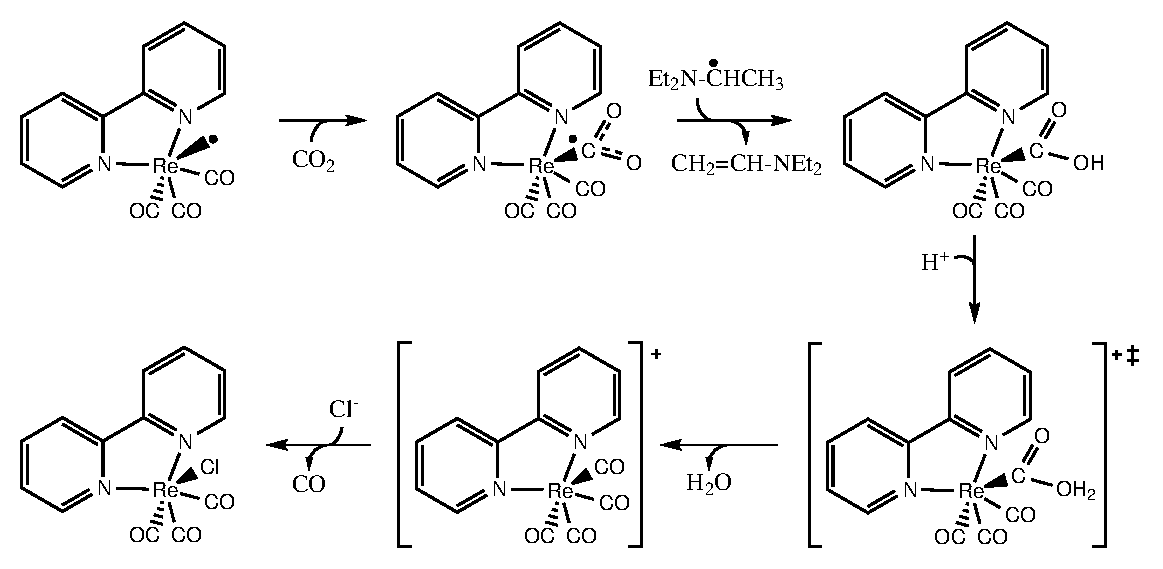
\includegraphics[clip=true, width=\textwidth, keepaspectratio]{images/watergas.eps}
 \end{center}
\caption{The `water-gas shift' mechanistic pathway}
\label{fig.watergas}
\end{figure} 

Energies of each of the compounds involved in this mechanism pathway are shown in \autoref{tab.wgsenergy}, along with the energy of solvation.

% Table generated by Excel2LaTeX
\begin{table}[!htb]
\centering
 \begin{threeparttable}
  \caption[Gas phase and solvated energies for the `water-gas shift' mechanism]{Gas phase and solvated energies of compounds, transition states and intermediates in the `water-gas shift' mechanism}
    \begin{tabular}{llrrr}
    \toprule
    Molecule & Label & E (gas)\tnote{a} & E (solution)\tnote{b} & E (solvation)\tnote{c} \\
    \midrule
    Catalyst-\ce{CO2} (Axial) & 4.31  & -1103.008904 & -1103.016031 & 4.47 \\
    Catalyst-\ce{CO2H} (Axial) & 4.32  & -1103.610331 & -1103.640451 & 18.90 \\
    \ce{H2O} Dissociation (Axial) TS & 4.33  & -1104.018352 & -1104.093313 & 47.04 \\
    Catalyst-\ce{CO2} (Equatorial) & 4.34  & -1102.963633 & -1102.992198 & 17.92 \\
    Catalyst-\ce{CO2H} (Equatorial) & 4.35  & -1103.597572 & -1103.625739 & 17.68 \\
    \ce{H2O} Dissociation (Equatorial) TS & 4.36  & -1104.016156 & -1104.093644 & 48.62 \\
    Water & 4.37 & -76.46413339 & -76.47581393 & 7.33 \\
    Tetracarbonyl Catalyst Cation & 4.38  & -1027.546073 & -1027.619412 & 46.02 \\
    H Transfer to Axial \ce{CO2} TS & 4.39  & -1394.981543 & -1395.011603 & 18.86 \\
    H Transfer to Equatorial \ce{CO2} TS & 4.40  & -1394.938949 & -1394.991623 & 33.05 \\
    Catalyst with Migrated Open Site & 4.41  & -914.2766988 & -914.2972247 & 12.88 \\
    \bottomrule
    \end{tabular}%
    \begin{tablenotes}
    \item [a] TPSS SCF energy in hartrees.
    \item [b] TPSS SCF energy in hartrees with COSMO solvation in DMF.
    \item [c] TPSS solvation energy in kcal/mol (E(gas) - E(solution)).
    \end{tablenotes}
  \label{tab.wgsenergy}%
 \end{threeparttable}
\end{table}%



% Table generated by Excel2LaTeX
\begin{table}[!htb]
\centering
 \begin{threeparttable}
  \caption{Energies for the reaction steps in the `formate' pathway}
    \begin{tabular}{rrrr}
    \toprule
    Description & Steps & Energy(gas)\tnote{a} & Energy(dmf)\tnote{b} \\
    \midrule
    Formation of Radical Anion & 2.1   & -39.271301 & -67.827267 \\
    Open site catalyst plus cl- & 2.2   & 50.8169125 & 15.4408871 \\
    Reconfiguration of TEA & 2.3   & -164.60991 & -118.34007 \\
    \midrule
    migration of open site? & 2.4   & 23.3674263 & 19.7662463 \\
    Addition of CO2 to open site & 2.5   & 4.78987184 & 1.56207334 \\
    H transfer to CO2 & 2.6   & -61.998066 & -35.596525 \\
    CO2H planar relaxation & 2.7   & 22.2489536 & -5.1943905 \\
    COOH2 ts & 2.8   & 144.908364 & 116.570584 \\
    CO4 + and water & 2.9   & 4.10436095 & -1.4970678 \\
    dissassotiation of CO & 2.10  & 40.893777 & 35.5673996 \\
    Reformation of Catalyst & 2.11  & -141.76995 & -36.367745 \\
    \bottomrule
    \end{tabular}%
    \begin{tablenotes}
    \item [a] TPSS SCF energy in kcal/mol.
    \item [b] TPSS SCF energy in kcal/mol with COSMO solvation in DMF.
    \end{tablenotes}
  \label{tab.wgsrxn}%
 \end{threeparttable}
\end{table}%




This mechanistic pathway it thought to start by the same addition of CO2 that is seen in the carbonate mechanism (see \autoref{ss.carbonate}, forming \textbf{4.31}. The added \ce{CO2} is able to extract a hydrogen from the once-reduced sacrificial amine \textbf{4.07}, allowing the completion of the ethene formation \textbf{4.26}. The newly formed acid species \textbf{4.32} dehydrates in the presence of a second proton (via \textbf{4.33}) to form water \textbf{4.37} and the tetracarbonyl cationic species \textbf{4.38}. 

Typically, this reaction had been thought to proceed on the axial site of the catalyst, mirroring the pathways discussed above. However, due to the ease of migration of the carbonyl groups, it is proposed that the `water-gas shift' mechanism does not occur entirely axial to the ligand, but begins with coordination of a \ce{CO2} molecule in between the \textit{facial}-\ce{CO} ligands, forcing a carbonyl to the axial position \textbf{4.34}. This \ce{CO2} bound in the plane of the ligand then undergoes hydrogen addition and dehydration to produce a molecule of \ce{H2O}, continuing as before. While any of the carbonyl groups could be labile, the carbonyl at the axial position is replaced by the halide to return to the starting catalyst\autocite{shaver1992}. 

\FloatBarrier

%---------------------------------------------------------------------
\subsection{Consequences From \texorpdfstring{\ce{$\kappa$^2}}{Bidentate} Terpyridine Complex Inactivity}
%---------------------------------------------------------------------

The lack of reactivity of the \ce{$\kappa$^2(terpy)Re(CO)3X} motif of complexes contrasting to the activity of the originally published \ce{$\kappa$^2(bipy)Re(CO)3X} indicates some influence of the ligand on the mechanism. While the terdentate complex can be rationalized to be inactive due to its short-lived excited state (as seen in the lack of fluorescence)\todo{fluorescence tests on 1,2}, this explanation does not suffice for the fluorescing bidentate complex. Other substituted bipyridine ligands are known to be active for photocatalytic reduction\todo{ref lehn88?}, identifying the most likely conflicting feature of the terpyridine ligand to be the pendant arm, and its availability for chelation to the metal centre. While in the radical eximer form, the chelation site is sterically blocked by one of the three carbonyl groups. However, reorganization of the substituent carbonyls from a \textit{facial} orientation to a \textit{meridional} could allow for the free pyridine to form the metal-ligand bond, resulting in compound (X)

% Table generated by Excel2LaTeX
\begin{table}[!htb]
\centering
 \begin{threeparttable}
  \caption{Energies for the reaction steps in the `formate' pathway}
    % Table generated by Excel2LaTeX from sheet 'Tex Charts
    \begin{tabular}{rrrr}
    \toprule
    Description & Steps & Energy(gas)\tnote{a} & Energy(dmf)\tnote{b} \\
    \midrule
    Formation of Radical Anion & 4.01, 4.05 \ce{->} 4.02, 4.06   & 124.261582 & 47.596907 \\
    Open site catalyst plus cl- & 4.02 \ce{->} 4.03, 4.04 & 50.816912 & 15.440887 \\
    Reconfiguration of TEA & 4.06, 4.05 \ce{->} 4.07, 4.08 & -1.077024 & -2.915901 \\
    \midrule
    Addition of CO2 to open site & 3.4   & -0.2501423 & 6.37310903 \\
    H transfer to CO2 & 3.5   & -19.133571 & -33.878805 \\
    CO2H axial relaxation & 3.6   & -0.2145456 & -1.1883574 \\
    COOH2 ts & 3.7   & 151.907871 & 125.579781 \\
    CO4 + and water & 3.8   & 5.1112987 & -1.2748062 \\
    dissassotiation of CO & 3.9   & 40.893777 & 35.5673996 \\
    Reformation of Catalyst & 3.10  & -141.76995 & -36.367745 \\
    \bottomrule
    \end{tabular}%
    \begin{tablenotes}
    \item [a] TPSS SCF energy in kcal/mol.
    \item [b] TPSS SCF energy in kcal/mol with COSMO solvation in DMF.
    \end{tablenotes}
  \label{tab.siderxn}%
 \end{threeparttable}
\end{table}%




%======================================================================
\section{Comparison Between Mechanistic Pathways} \label{sec.compare}
%======================================================================

Previous studies in literature had only analyzed one possible mechanistic pathway (or a subsection thereof), without a fuller analysis of the competitiveness of each pathway relative to the others. Discussion on the tenability of each potential pathway relied on the \textit{in situ} observation of intermediates or transition states, the success (or lack thereof) of synthesis of the intermediates, and the relative production of by-products in the mechanistic trials.

The overall energies for each of the mechanistic pathways shown in \autoref{fig.threepath} are shown in \autoref{fig.threeenergies}. 

\begin{figure}[!htbp]
 \begin{center}
  
\includegraphics[clip=true]{images/insertgraphic.eps}
 \end{center}
\caption[Reaction energies for three mechanistic pathways]{An overview of the energies of the three mechanistic pathways of photochemical \ce{CO2} reduction}
\label{fig.threeenergies}
\end{figure} 
\todo{SOLVE ENERGY}

%======================================================================
\section{Conclusions} 
%======================================================================

With the energies of each of the independent mechanisms elucidated, the feasibility of each mechanism becomes evident. Evidence in literature suggests that all mechanisms progress to some degree, however, the production of \ce{CO} outpaces that of the partial reduction or oxidation pathways. 
